\documentclass[10pt, author, twocolumn]{article}

\usepackage{subcaption}
\usepackage{pdfpages}
\usepackage[margin=1in]{geometry}

% Author Information
\title{\vspace{-0ex}Bench: Evaluating Arbitrary Workloads}
\author{Yash Gupta \\
ygupta@ucsc.edu}
\date{\vspace{-3ex}}

\begin{document}
\maketitle
	
\begin{abstract}
Software applications use medium like HDD (Hard Disk Drives) and SSD (Solid State Drives) to store information and data. The storage workloads for these applications vary, ranging from highly sequntial workloads to ones which utilize the drives in a random order. Choosing the correct medium of storage is essential to delivering optimal performance for these applications. Hence, it is crucial to benchmark these workloads to identify the most suitable storage medium. Furthermore, it is important in general to recognize which workloads suit a specific storage medium the most. The work presented in this paper introduces an application "bench" which provides a way to benchmark these varying types of workloads using a consumer/producer architecture. Using \textit{bench}, we evaluate and present the result of some common industrial workloads and their performance metrics on a variety of storage medium.
\end{abstract}

\section{Introduction}
Most computer algorithms utilize the storage disk inside of a system. While some access the disk directly, as in the case of data structures like B-Trees and LSM-Trees \cite{o1996log}, others may end up accessing them indirectly, perhaps through the means of a paging algorithm in a virtual memory system. These algorithms effectively define a workload which is to be executed by the system. More often than not, the storage medium of a system is the main bottleneck which limits the performance of this workload on any given system \cite{smith1985disk}. This is not hard to believe, particularly because the performance differences between commodity storage media like HDD and SSD pale in comparison to CPU, RAM, and even networking nowadays \cite{boden1995myrinet}.

To be able to reduce or even elminate this bottleneck, it is critical to realize which class of storage media technology performs most efficiently for a given workload. Using this information, one can make better decisions with regards to system design and provide a more definitive performance analysis for the overall system. However, all algorithms produce different workloads and in most cases, a software application itself employs many different algorithms. Hence, it makes more sense to refer to a workload as part of an application rather than that of an algorithm. This abstraction is also extendable to systems which employ different sets of applications to provide some service, an example being an operating system such as Unix. In such a case, workload may refer to the overall workload of the operating system rather than the seperate workloads of the applications within it.

Keeping this in mind, it is important to understand that different storage media performs differently for particular types of workloads. Conventional rotating media like hard disk drives perform optimally in a sequential workload, whereas flash based storage such as used in solid state drives can perform admirably even in a random-heavy workload. However, flash based storage costs more than rotating media storage per giga byte. This means that an engineer designing a system needs to make careful decisions on the inclusion of hard drives, solid state drives and even a combination of both. Driving these decisions is usually a benchmark, highlighting the performance and cost characteristics of the different types of storage media. However, performing such an exhaustive benchmark is a non-trivial task. Different classes of applications produce completely different workloads. For example, a web page may produce small-random oriented workloads whereas a paging algorithm for an operating system might produce a long-sequential one.

In this paper, we present a benchmarking application called \textit{bench}, which uses a probability distribution of random and sequential I/O, along with an exponentially distributed arrival interval to simulate the arrival of work. We argue that such a benchmarking architecture is capable of evaluating any arbitrary workload, as every storage workload can be dissolved into these primitives. We then use \textit{bench} to evaluate benchmarks of some common industrial workloads such as database processing, file transferring and memory paging. 

The rest of the paper is structured as follows: Section 2 provides a background on the different types of storage media used in industrial applications. Section 3 explains the design of \textit{bench} and section 4 explains its implementation. Section 5 discusses the evaluation of certain workloads performed using \textit{bench} and finally, section 6 concludes the paper.

\section{Background}

The two most common options used for industrial storage comprise of rotation based media, such as hard disk drives, and flash based media, such as solid state drives. Both of these media have their sets of pros and cons which make them suitable for different kinds of workloads. For industrial class applications, the choice of choosing between these media is crucial as they are tailored to different circumstances and situations. This section provides differences between the two along with some of their assumed performance characteristics. 

\subsection{Rotating Media}

For the purposes of this paper, the only rotating media we consider is a hard disk drive. While there are other rotating storage media such as a Compact Disk (CD), they are not usually used for long term storage, and hence, they do not make a viable option for large scale storage systems.

Most of the information on HDDs presented here is a paraphrasing of \cite{osbook}. For readers looking for a more in-depth and technical explanation for the working of disk drives, chapter 37 in the book provides a solid ground. 

The core concept behind the working of a disk drive is magnetization. Each disk drive has a set of \textbf{platters}, which are smooth, double-sided surfaces. These platters are usually made of aluminum and are coated with a thin magnetic layer. The idea is that this layer can be magnetized to store bits, enabling the platter to store bits even when the disk drive in turned off. This is due to the fact that the magnetic layer does not lose its magnetization upon the loss of current. 

All the platters in a disk drive are organised as a set of concentric circles, each of which is known as a \textbf{track}. These tracks are then further divided into smaller regions called \textbf{sectors}, and the sector size denotes the granularity of I/O for any given disk drive. The tracks on a platter are packed together incredibly tightly, with hundreds of tracks fitting within the width of a human hair.

The disk platters themselves are attached to a \textbf{spindle}, which in turn is connected to a motor which spins at an incredibly fast rate. It is typical for modern disk drives to have rotations in the range of 7200-15000 RPM (rotations per minute). 

Finally, for reading or writing to the disk, a \textbf{disk head} (attached to a \textbf{disk arm}) is used. This head hovers just slightly above the platter, and is free to move between the different tracks. The head is able to read the magnetic nature of the layer at its position, sensing whether it is north or south. It is also capable of changing this nature by applying a focused magnetic field, hence providing it the ability to write a bit onto the platter.

Due to this design, disk drives suffer from costly operations known as \textbf{rotational delays} and \textbf{seek time}. Rotational delays are the delays encountered when the disk head needs to wait for the correct sector within a track to come under it. Seek time on the other hand is the time it takes for a disk head to move to another track on the platter altogether. Both of these operations incur a heavy time penalty, and even though certain optimizations have been made to reduce their cost (such as track skewing), they remain the leading cause of slower disk performance. 

One particular area where disk drives are notoriously bad in terms of performance is small, random I/O. For any I/O request, disk drives perform better if the sectors to be read are closer together. Moreover, as each request incurs overhead from seeking and rotating, having a large number of small requests means that the overhead penalty is experienced more often. Owing to these factors, it is natural to believe that long sequential I/O is more suited to disk drives as it largely avoids the overhead penalty of seeking and rotating. 

Another noted downfall of disk drives is the involvement of moving mechanical parts, such as the disk arm, which often break down and require repair and replacement.

\subsection{Flash Media}

Flash memory is a subset of EEPROM (electrically erasable programmable read-only memory). While there are two types of flash memory, namely NAND-flash and NOR-flash, this paper focuses on NAND-flash as it is the more commonly deployed variant \cite{micheloni2010nand}. Hence, further mentions of flash memory within this paper refer to the use of NAND-flash class of technology. 

There are several different types of storage technologies built on top of flash memory. Some examples include solid state drives, usb-drives, and micro SD cards. This paper provides a general background on flash memory, as the foundation for all these flash storage technologies is largely the same. Our benchmarks focus only on solid state drives however, as they are more commonly deployed that other flash technologies.

The main idea behind flash memory is the use of floating-gate transistors \cite{micheloni2010nand}. Without diving into too much detail, the basic idea involves detecting the presence of a charge in a \textbf{flash cell}. When a certain voltage is applied to parts of the cell, current is allowed to flow through the transistor. We can detect the charge present in the cell by monitoring this current, allowing us to judge the current state of the cell \cite{micheloni2010nand}. When an even greater voltage is applied, a process known as quantum tunneling allows us to trap an electron in the transistor, allowing us to effectively change the charge of the cell and write a single bit of information to it.

Flash memory groups a set of these cells into \textbf{pages}. A single page is the granularity for reading and writing to flash memory, and in general, page size is set to 4 KB. One problem with flash memory is that a page cannot be written to unless it has been previously erased. Unfortunately, flash memory performs the erase operation on a \textbf{block} granularity. A block is a collection of pages and usually block size is much greater than page size. The reason that this is the case is because the erase operation consumes a lot of voltage, which in turn consumes more power and at the same time damages the structure of the transistor in a cell. Hence, an erase operation batches a number of pages together and erases them all at the same time. While this improves the endurance and performance of flash memory, the assymetric granularity of writes and erases create an interesting problem: updates to flash memory cannot be done in-place.

A proposed solution to this problem is the use of management firmware known as a \textbf{flash translation layer (FTL)} \cite{kim2002space}. An FTL essentially provides a mapping from logical addresses (which are visible to a host system) to physical addresses (which are not visible to a host system) on the flash chip. In an example FTL, if a host were to randomly update a single page in flash memory, the FTL would copy the entire block which contains the requested page over to another place in flash memory, making sure to replace the original page with the modified one. It would then change its mapping table, establishing the new mapping of logical to physical addresses. By doing this, the FTL can avoid erasing blocks frequently, increasing the lifetime of the flash memory. Unfortunately however, in this case, the flash memory incurred a lot more writes than intended, increasing the write latency and decreasing overall throughput. This phenomenon is known as \textbf{write amplification} (WA) and a lot of research has gone into building FTLs which can provide lower write amplification. Regardless of any progress on that front however, write amplification continues to be a major bottleneck for flash memory and prevents random writes (which incur heavy write amplification as explained above) to perform efficiently.

Owing to such characteristics, flash aware software systems have begun using different design paradigms to optimize the use of flash memory. One such example is the use of log based structures wherein all information and operations are performed as appends to a file, making sure that previously written pages are not updated further \cite{rosenblum1992design}. 

An important thing to note is that flash memory performs admirably for random reads when compared to disks because it incurs no overhead from rotations and seeking. However, there are physical challenges which prevent flash based storage to provide the same capacity as disk \cite{micheloni2010nand}. As a result of that, flash storage is more expensive than disk based storage and requires novel techniques to make it viable for the enterprise \cite{colgrove2015purity}. 

\section{Design}
We have designed \textit{bench} with keeping this background in mind. In this section, we explain the design choices made for \textit{bench}. We argue that these design choices allow \textit{bench} to benchmark most if not all types of workloads. By using a probability distribution for tasks and an exponential distribution for arrival time, along with a simulated distributed environment, \textit{bench} is theoretically capable of modelling most industrial workloads. 

\subsection{I/O Task}
Before we begin to explain the design of \textit{bench}, it is important to understand certain storage primitives such as an \textbf{I/O Task}. Any I/O to a drive will consist of either \textbf{read} or \textbf{write} operations. These operations fall within two I/O classes, namely \textbf{random} and \textbf{sequential}. 

An I/O task is essentially a tuple which describes an I/O operation of a certain size at a specific offset in the drive. Depending upon the relation of this I/O task to previous I/O tasks, it may be classified as either random or sequential. Random I/O is usally smaller in size and in most cases bears no correspondance to previously issued I/O tasks in the system. Sequential I/O on the other hand is usually larger and has a direct correspondance to previously issued tasks. For example, consider a workload which reads a drive at 1 MB per read request. If the first read for the workload takes place at offset 0, then the next sequential read will take place at offset 1 MB. On the other hand, if the workload processed reads randomly, then such a correspondance between the two read requests wouldn't likely exist. While this assumption is not always true, it is a fair one to make.

Based on this primitive of an I/O task, we can break down any given workload into a list of I/O tasks it performs. Using this list, we can build a distribution which describes the probability of each type of task occuring. This distribution is simple to build as there are only four types of I/O tasks: random read, random write, sequential read and sequential write. If an application was to process this list, then it would execute the same workload as the original application, albeit without any application context. While not having context generally makes no difference to most workloads, it makes accurately benchmarking certain workloads difficult.

Consider a workload which processes I/O tasks with a very strict order. A random read in this workload is followed by a sequential write, which is then followed by a random read and so on. While it is possible to benchmark such a workload through a probability distribution, a benchmark based solely on task distribution will be inaccurate as it will not be able to guarentee the order of the tasks. Future versions of \textit{bench} aim to find a workaround.

\subsection{Arrival Time}
Besides the task distribution, this is another challenge benchmarking applications face. \textit{How to accurately model the arrival of work, or in layman terms, how does a benchmarking application know when a client has arrived?}. 

It is inaccurate to assume that an application is always busy. Conversely, it is also inaccurate to assume that an application is never busy. Moreover, even if one knows the average arrival time of clients for an application, it is inaccurate to assume that the application processes the clients at constant intervals. However, there is a statistical distribution which has been proven to model interval times between discrete events accurately. \textit{bench} uses this distribution as a basis for arrival times of work. 

A \textbf{Poisson point process} is a process in which events occur continously and independently at a constant average rate \cite{kingman1993poisson}. This means that as time $t \Rightarrow \infty$, the average of the intervals between events in a point process converge. Hence, for a system with a known average, \textit{such as a workload}, the poisson point process can model the interval times between a pair of events. An \textbf{exponential distribution} is the probability distribution which describes an interval between a pair of events in a poisson point process \cite{buzen1973computational}. Hence, using an exponential distribution, we can accurately model the arrival of work for any given workload.

However, this approach is not perfect. Suppose a workload experiences different arrival times under different curcumstances, such as time of day. A workload which experiences a different arrival time of clients between day and night cannot be modelled correctly with an average. The average shadows the different stress levels which the workload produces and coalesces them into a single, more normalized arrival time. This can lead to inaccurate benchmarks. We aim to solve this issue in future revisions of \textit{bench}.

\subsection{Distributed Architecture}
Most industrial applications are built as distributed systems which divide work amongst different entities in order to better process requests from clients. In a generic distributed application, a frontend system collects a request from a user and forwards it to a backend system. This backend system processes this request and ships the information back to the frontend or to the client. 

The reason this system is as such is because industrial applications operate at a huge scale and service thousands of requests at a given time. It is simply not possible for a single machine to keep up with the incoming requests from impatient clients. For a system such as this, the main bottleneck used to be the latency of network connections which connected the frontend to the backend. However, with advances in network technology and the introduction of standards such as \textbf{Infiniband} \cite{pfister2001introduction}, this is not true anymore. Instead, the main bottleneck for these systems is the storage media, which operate at a fraction of the speed of CPU and RAM. 

As the network is not a bottleneck anymore, we decided that we can combine the frontend and the backend into a single application and simulate them using threads instead of building two separate applications, one for the frontend and one for the backend, and then connect them together using a network simulator. We claim that having two separate applications because of something which as is does not limit performance provides no benefit to having an application which simulates entities using threads. Infact, we argue that bulding separate applications leads to more bug prone software and will overall provide deprecating results. 

Moreover, we decided that a single instance of \textit{bench} will only benchmark a single workload. We pin each entity to its own thread and so benchmarking multiple workloads simply means more threads. As the relative overhead of setting up an entity is small, having separate instances represent different workloads is not any more costlier and provides a cleaner, more manageable design. 

\section{Implementation}
Our goal was to make \textit{bench} an easy to use and flexible application. As \textit{bench} requires heavy parametrization due to its design, we decided that the best way to build it is to divide the application into modules and then build the modules in a language most suitable for it.

As processing of workloads requires multiple threads and low level disk access, we decided that the core benchmark engine should be built in \textbf{C}. Meanwhile, we used \textbf{python} to build a script to handle the higher level tasks such as parsing arguments and building graphs. We defined a file format which neatly collects all the benchmark variables such as task distribution and the python script reads in such a file and then forwards these variables as a tuple to a compiled binary in the form of program arguments. From there, the benchmarking engine takes over and begins the benchmark. 

\subsection{Work Profiles}
\textit{bench} represents a given workload as a \textbf{work profile}. A work profile is essentially a structure which comprises of the tunable knobs for the benchmark. These include the distribution of the types of I/O, along with a respective size for them. 

Work profiles store the probability distribution of the tasks using a cumulative distribution sum and intervals within this sum represent the task. For exmaple, consider a workload with the following distribution: random read (50\%), random write (10\%), sequential read (15\%) and sequntial write (25\%). The work profile will store these as: random read ([1, 50]), random write ([51, 60]), sequential read ([61, 75]) and sequntial write ([76, 100]). Now, to generate a task with respect to the distribution, all we need to do is generate a uniformly distributed random number $x$ in [1, 100]. Depending on the interval bracket $x$ falls in, we choose a size and an offset for the I/O task. 

If a task is random, then a random offset is generated in [0, DRIVE\_SIZE-TASK\_SIZE]. In case the task is sequential, then the next corresponding offset is calculated with the help of static variables. So for the previous example, if the random read size was 4 KB and $x = 20$, then a random offset will be generated in [0, DRIVE\_SIZE-4096] and this offset will be paired with the 4 KB size in a tuple and sent forward for processing.

The current implementation of \textit{bench} uses \texttt{rand()} from the standard library to generate random numbers. We are aware of the fact that \texttt{rand()} has shown to \textbf{NOT} be uniformly distributed. For future versions, we are looking into using the linux system call \texttt{getrandom()} as our entropy source. 

\subsection{Multithreading}
We implemented the simulation of a distributed system using the \texttt{pthreads} library in \textit{bench}. The idea is that we have a \textbf{producer} thread and a \textbf{consumer} thread (which simulate a frontend and a backend respectively) which are both managed by a \textbf{timer} thread. The timer thread works in tandem with the consumer thread to enforce an order of termination between the consumer and the producer thread. If this order is not followed, the application may reach a state where the consumer sleeps for an indefinite amount of time. This is explained further in the following paragraphs.

The producer has a relatively trivial task compared to the consumer. It simply executes an infinite loop with these instructions: 

\begin{enumerate}
    \item Acquire an exponential variate of the arrival averge in microseconds. Let this be $n$.
    \item Call \texttt{usleep} with $n$ as the parameter. 
    \item Upon waking up, generate an I/O task and append it to the circular queue shared with the consumer. 
    \item Repeat. 
\end{enumerate}

The consumer on the other hand does a lot more. Its workflow is divided into separate phases which are represented using an \texttt{enum}. They are: \texttt{initialize}, \texttt{process} and \texttt{output}. The initialize phase is for setting up allocations and opening the required file descriptor. The process phase is a loop which processes I/O tasks acquired from the circular queue. Finally, the output phase is where the consumer dumps all statistically relevant information for making the performance graphs. 

The reason the consumer is much more complex and requires these phases is because unlike the producer thread which outputs nothing, the timer thread cannot simply call \texttt{pthread\_cancel()} on the consumer as the consumer needs to output data it acquires during the processing phase. This is also the reason the timer thread needs to enforce a termination order between the producer and the consumer. 

Consider a situation where the circular queue is empty and the consumer goes to sleep, hoping the producer will wake it up. If the timer thread cancels the prodcuer before it can wake the consumer up, then the consumer sleeps indefinitely and the only way to come back to a workable state is to manually kill the program. To avoid such a situation, the following ordering policy takes place:

\begin{enumerate}
    \item The timer thread signals the consumer using a global variable to changes its state from process to output. 
    \item Once the consumer acknowledges the signal and exits the processing loop, it sends a confirmation to the timer thread. 
    \item Upon receiving the confirmation, the timer thread calls \texttt{pthread\_cancel()} on the producer and then calls a \texttt{pthread\_join()} on the consumer.
    \item After the consumer finishes the output phase, it exists cleanly and the join in the timer thread returns. 
\end{enumerate}

By enforcing this order, the producer thread stays active for as long as the consumer might require it and hence, we can avoid the indefinite sleep problem. 

\subsection{Graphs}
The consumer collects a lot of data during its process phase. All of this data is outputted to a file during the output phase. The python phase which started the benchmark parses this file and uses the \texttt{plotly} module to build graphs from it.

We decided to use the \texttt{matplotlib} module over the more commercial \texttt{plotly} module as, in out opinion, graphs from the \texttt{matplotlib} are more visually appealing.

\section{Evaluations}
In this section, we present our evaluations taken using \textit{bench}. We evaluated a standard industry benchmark which evaluates the performance of storage media for a web server. The workload for this is as such: random read (65\%, 4 KB), random write (10\%, 4 KB), sequential read (20\%, 64 KB) and sequential write (5\%, 64 KB); Arrival time: 0.1 seconds. This was evaluated on a Western Digital 1TB HDD and a LITEONIT 80GB mSATA SSD.

We also evaluated standard benchmarks to corrobate the performance characteristics of chosen media. Hence, we chose a sequential based workload for the HDD and sequential + random read based workload for the SSD. 

\begin{enumerate}
    \item Sequential: random read (0\%, 64 KB), random write (0\%, 64 KB), sequential read (70\%, 64 KB) and sequential write (30\%, 64 KB); Arrival time: 2 seconds. \textbf{This is a close modeling of a virtual memory paging workload}.
    \item Sequential + Random Reads: random read (20\%, 16 KB), random write (10\%, 16 KB), sequential read (30\%, 128 KB) and sequential write (40\%, 128 KB); Arrival time: 2 seconds. \textbf{This is a close modeling of a log structured FS}.
\end{enumerate}

\subsection{Web Server}
The evaluations for the web server benchmark highlight that while the SSD performs better than an HDD (Figures 1, 2, 4 \& 5), they both have similar characteristics for the workload. This means that if we had an HDD which has similar performance ratings as the SSD, then the HDD would perform just as nice as the SSD for this workload. 

\subsection{Paging and LFS}
From the paging graphs (Figures 3 \& 6), an HDD achieves high throughput and low latency for both I/O tasks. On the other side, an SSD does amazingly well for an LFS workload, with sequential read throughput crossing 300 MB/s (Figures 7 \& 8). 

These sets of graphs confirm the performance characteristics of these storage media and should vouch for \textit{bench} being a viable benchmarking application.

\section{Conclusion}
It is possible to build a benchmarking application capable of benchmarking most if not all workloads. The corroboration of the result with the expectation means that \textit{bench} is a viable option for performing becnhmarks on workloads. 

Some future work includes expanding the probability distribution to include certain predicates which may make it possible to address some of the highlighted issues. We are also looking into predicates for arrival times, which should rectify the inaccuracies of an overall average arrival time.

\newpage
\begin{figure}[t!]
    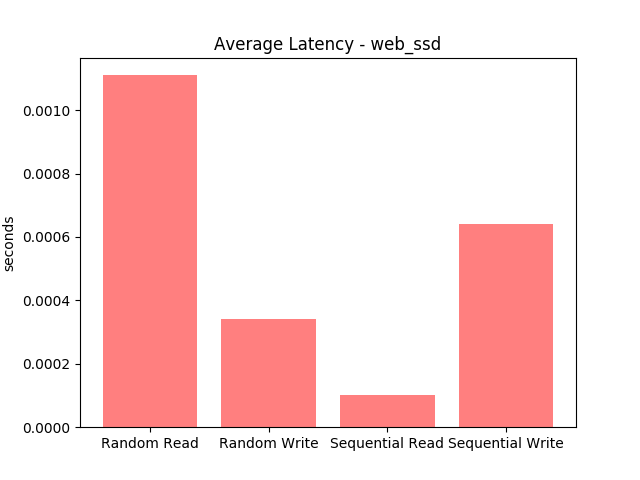
\includegraphics[scale=0.5]{../graphs/web_ssd-lat.png}
    \caption{Web Server Latency (SSD)}
    \label{fig:ssd_web_lat}
\end{figure}

\begin{figure}[h!]
    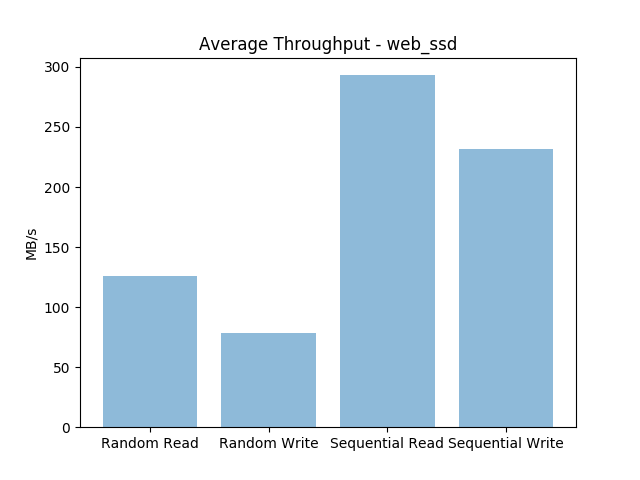
\includegraphics[scale=0.5]{../graphs/web_ssd-thru.png}
    \caption{Web Server Throughput (SSD)}
    \label{fig:ssd_web_thru}
\end{figure}

\begin{figure}[h!]
    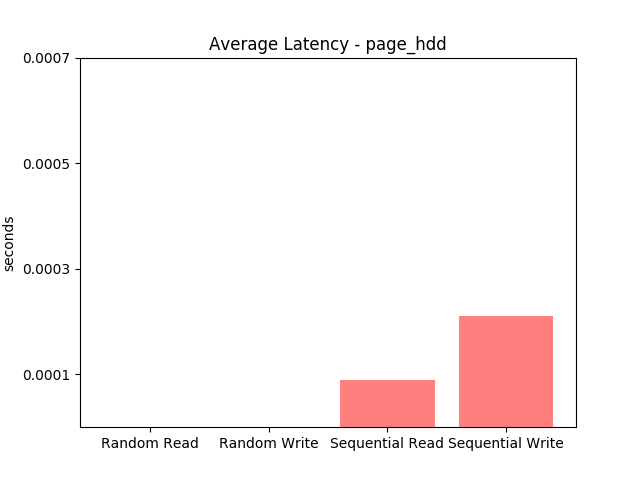
\includegraphics[scale=0.5]{../graphs/page_hdd-lat.png}
    \caption{Page Workload Latency (HDD)}
    \label{fig:hdd_page_lat}
\end{figure}

\begin{figure}[h!]
    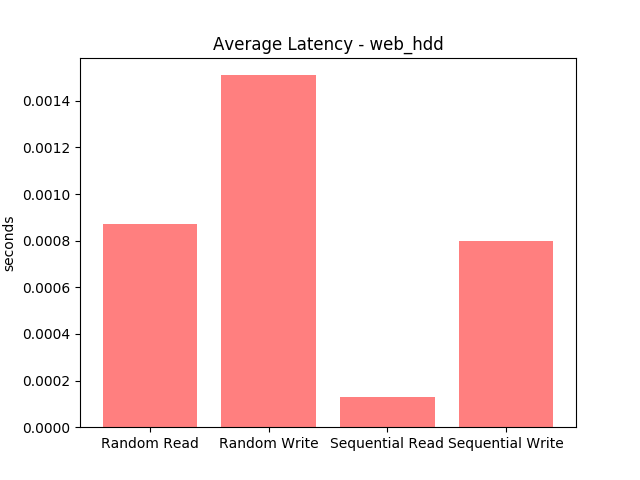
\includegraphics[scale=0.5]{../graphs/web_hdd-lat.png}
    \caption{Web Server Latency (HDD)}
    \label{fig:hhd_web_lat}
\end{figure}

\begin{figure}[h!]
    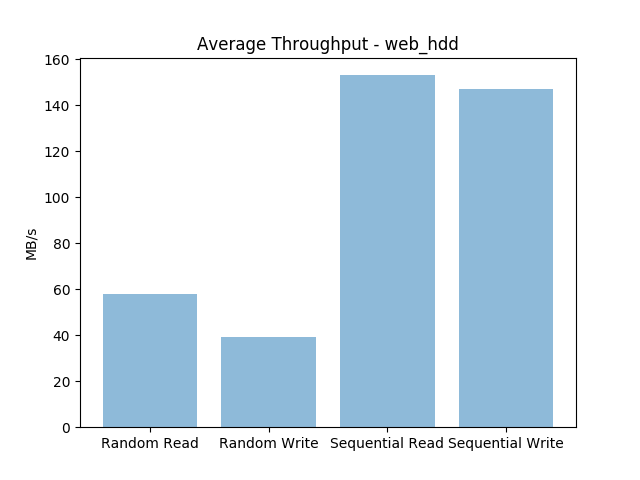
\includegraphics[scale=0.5]{../graphs/web_hdd-thru.png}
    \caption{Web Server Throughput (HDD)}
    \label{fig:hdd_web_thru}
\end{figure}

\vspace{5cm}
\begin{figure}[h!]
    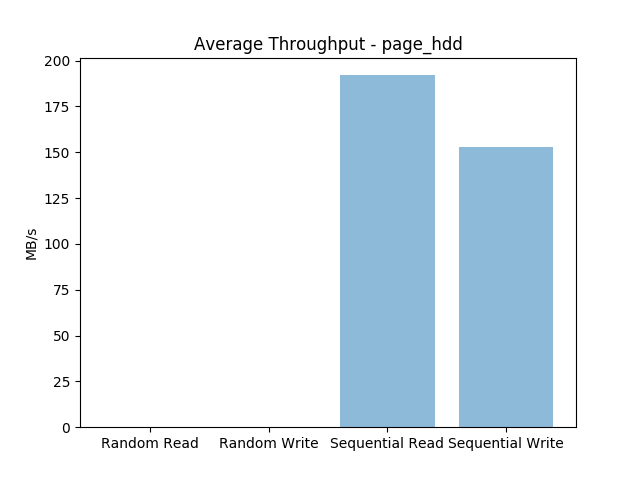
\includegraphics[scale=0.5]{../graphs/page_hdd-thru.png}
    \caption{Page Workload Throughput (HDD)}
    \label{fig:hdd_page_thru}
\end{figure}

\begin{figure}[t!]
    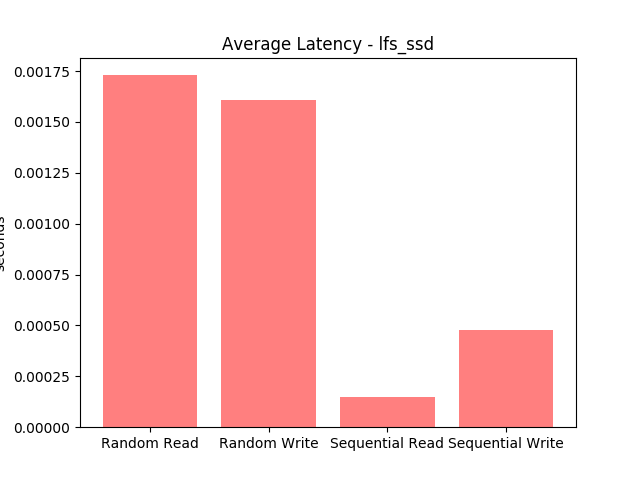
\includegraphics[scale=0.5]{../graphs/lfs_ssd-lat.png}
    \caption{LFS Latency (SSD)}
    \label{fig:ssd_lfs_lat}
\end{figure}

\begin{figure}[t!]
    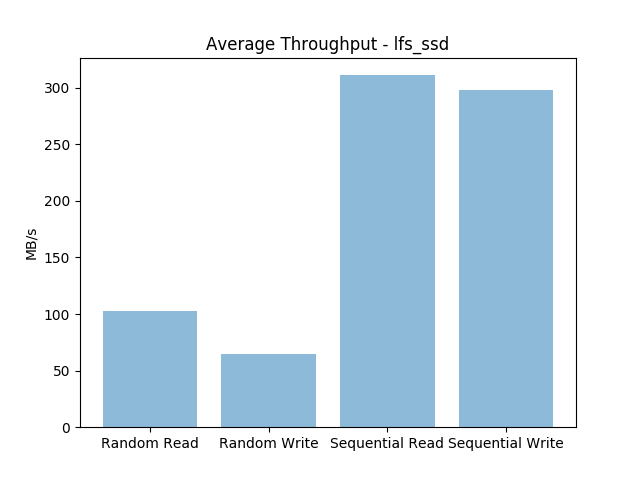
\includegraphics[scale=0.5]{../graphs/lfs_ssd-thru.png}
    \caption{LFS Throughput (SSD)}
    \label{fig:ssd_lfs_thru}
\end{figure}

\bibliographystyle{plain}
\bibliography{cites}

\end{document}